\subsection{Detector Effects}
\begin{figure}
\centering
\includegraphics[width=.5\textwidth]{figures/AGIPD.png}
\caption{Application Specific Integrated Circuit of a single pixel of the AGIPD detector with storage pipeline. Source: \cite{henrich2011adaptive}.}
\label{abb. AGIPD}
\end{figure}
Particle detectors are complex electronic devices ranging from
transistors to \glspl{apic}
\cite{potdevin2011analysis} \cite{shi2010challenges}. Due to imperfections in
the material those circuits bear a natural source of fluctuations. Especially,
the influence of leakage currents on operation amplifiers that increase with
radiation intensity can result in increased noise levels
\cite{shi2010challenges}. The resulting noise is often still
smaller than e.g. the statistical fluctuations in the photon number in each
pixel \cite{shi2010challenges}.

Furthermore, leakage currents from another origin are much more serious. Since
the XFEL source produces more images than can be processed in one of its
\SI{600}{\micro\second} pulse trains, the detector needs to store those image values previous
to processing in a pipeline for each pixel (see figure \ref{abb. AGIPD}). After
each of those pulse trains there is a gap of approx. \SI{100}{\milli\second}, where the detector
reads the pixel values of all stored images, digitizes them and store them on a
hard disk. This pipelines consist of capacities and switches that suffer from
leakage currents, as well. This not only affects the output values of intensity
but also the noise level of the readout and digits \cite{shi2010challenges}.

Detectors at European XFEL have to cope with a very complex parameter space.
They have to cover a broad range of energy of many \si{\kilo\electronvolt} for every pixel
independently of each other. Furthermore, the pulse rate of the recording is
quite high. Additionally, they need to be sensible enough to detect single
photons but robust enough not to be destroyed at high intensities. This requires
protection of the electronics leading to additional readout noise
\cite{potdevin2011analysis}. Despite optimizations, detectors have a finite
dynamic range of values, which, once exceeded, leads
cut--off signals \cite{potdevin2011analysis}.

Additionally, there
are also physical effects producing noise. Thermal fluctuations can be reduced
by cooling. However, high intensity radiation can create plasmas in detector
pixels that effect neighbouring pixels due to electron drift
\cite{potdevin2011analysis}. The process is called ``blooming'' and is
taken into account in the charge simulation of this detector simulation project.
Additional information can be found in references: Joy et al. \cite{Joy2015},
R\"uter et al. \cite{Rueter2016}, Shi et al. \cite{shi2010challenges} and Potdevin et al. \cite{potdevin2011analysis}.

Last but not least, the number of photons arriving at a pixel and the number of
charges created from an interacting photon are statistical values. They are
uncertain and follow the Poisson statistics. Together with the blooming this
makes up the most important source for noise. Nevertheless, in many experiments
the noise resulting from a well optimized detector is much less than the
fluctuations in the signal resulting e.g. from optical
elements\cite{potdevin2011analysis}.
%
\subsection{Existing Software}
\subsubsection{Geant4/ X--CSIT}
%
\begin{figure}
  \centering
  \includegraphics[width=0.6\textwidth]{figures/XCSIT.png}
  \caption{Schema of the different parts of the detector simulation software \textit{X--CSIT}. Source: \cite{Joy2015}.}
  \label{abb. XCSIT}
\end{figure}
%
For the simulation of detectors Joy et al.~\cite{Joy2015} have
created an object oriented software library in the C++ programming language,
called \textit{X--CSIT}\footnote{\textit{X--CSIT} is not free software, hence access
is limited to users who have access to the European
XFEL gitlab repository.}, to simulate the behaviour of 2D semiconductor pixel detectors. Due to
the object orientation not only the initally implmented LPD, AGIPD, DCCS, pnCCD
and FastCCD detectors but also derived detectors can be supported
\cite{Joy2015}. Initially written for being integrated into the \textit{karabo}
framework, the software is universal enough to be stand--alone.

\textit{X--CSIT} consists of three parts \cite{Joy2015} as can be seen in figure
\ref{abb. XCSIT}. The first one, the particle simulation, describes how
photons interact with the active layer of the detector. For this purpose
\textit{X--CSIT} acts as a wrapper of the interaction simulation software
\textit{Geant4} \cite{Joy2015}. \textit{Geant4} covers the physical models of a
broad range of energy ranging from \si{\kilo\electronvolt} to
\si{\tera\electronvolt}~\cite{agostinelli2003geant4}. The
models can handle electromagnetic processes such as the photo electric
effect and fluorescence but also hadronic and optical processes. The standard
processes such as photo electric effect, Compton and Rayleigh scattering, as well
as Auger processes are also included \cite{Joy2015,agostinelli2003geant4}.
For this part \textit{X--CSIT} has the task to
manage the data transfer from and to \textit{Geant4}.
%
\begin{figure}
  \centering
  \includegraphics[width=0.6\textwidth]{figures/ChargeSpread.png}
  \caption{Sketch how a charge cloud produced from a single interaction can
    spread to neighbouring pixels. Source: \cite{Joy2015}.}
  \label{abb. Spread}
\end{figure}
%
The second part, the charge simulation, deals with the propagation of the
charges and plasmas created by interactions. Their behaviour is mainly governed
by drift and diffusion of electrons which can be described with a Gaussian
normal distribution (see figure \ref{abb. Spread}) with the following standard
derivation \cite{Joy2015}:
%
\begin{align}
  \sigma_{d} = \sqrt{\frac{2k_{\text{B}} T}{q E} \cdot d}.
\end{align}
%
Here $d$ is the depth in the material, $T$ the temperature, $q$ the drifting
total charge and $E$ the electrical field that pulls the charge to the readout
electronics of the detector.

The last part of \textit{X--CSIT} covers the detector readout electronics.
The electronic simulation simulates the electronic components of the detector
and their behaviour. For this purpose, \textit{X--CSIT} offers modules which are
combined to represent the circuits of the detector \cite{Joy2015}. This
simulation is not included the detector simulations for \textit{simex\_platform} because it
requires a tight connection to, e.g., the calibration software and database for
specific detectors.
%
\subsection{Extending C++ to Python}
Since \textit{X--CSIT} is written in C++ and the calculators of the
\textit{SimEx}\footnote{\textit{SimEx} is the python library inside the simulation
environment \textit{simex\_platform}} are written in python, there is a need of extending C++ classes
to python. To extend the X--CSIT classes to python, we used the
\textit{boost.python} library
(\url{http://www.boost.org/doc/libs/1_65_0/libs/python/doc/html/index.html})
\textit{Boost.python} consits of
header files that need to be added to the C++ implementations. Additionally, in
a BOOST\_PYTHON\_MODULE needs to be defined. This
module creates the equivalent of a python module and needs to define all the
extended classes, their functions as well as their return and input parameters
explicitly \cite{boostpython}. Consequently, \textit{boost.python} can be seen
as a module including abstract types that can be linked to C++ instances as well
as to python instances.

\subsection{Design}
%
\begin{figure}
  \centering
  \includegraphics[width=.99\textwidth]{figures/Design.png}
  \caption{Sketch showing the dependencies and inheritance structure of the py\_detector\_interface. Colour code: yellow $\hat{=}$ classes written in python, blue $\hat{=}$ classes written in C++, red arrows $\hat{=}$ inheritance, green arrows $\hat{=}$ manipulation of other instances, black arrows $\hat{=}$ data flow.}
  \label{abb. design}
\end{figure}
Since C++ and python programming languages belong to the object oriented
programming languages, the concept of inheritance and polymorphism are well
suited to achieve the desired extension and integration.
Polymorphism is the key concept for using self written
classes of this design in \textit{X--CSIT}. It allows also to minimize redundant
source code that is always a potential source of error and very difficult to
maintain. However, the required features remain accessible. For this reason, all
the created classes except \textit{Constants} are derived from \textit{X--CSIT}
or \textit{SimEx} base classes and interfaces as can be seen in figure \ref{abb.
design}.

Another important aspect of this design is the design of the python class. In
the end, this is the class that is accessed and used for performing the
simulation. For this reason, it should have control over input and output as
well as control over running the simulation. As can be seen in figure \ref{abb.
design}, the \textit{XCSITPhotonDetector} calculator is given control over each
step of the simulations. This includes creating data containers, initiate and
run the simulations as well as reading the input file and creating the output
file.

Nevertheless, the simulation itself should be triggered from C++ code. One
reason for this is that tunnelling through the \textit{boost.python} layer is
assumed to be slow. Additionally, python code is slower than C++ and there where
additional features needed such as a changed function signature in
\textit{ChargeSim}. Consequently, setting up and running simulations is
programmed in C++ and only calling these functions is extended to python.

Last but not least, the entire project needs to be integrated into
\textit{simex\_platform}. With regard to the source code style and function this can
easily be achieved by applying inheritance. However, one does not want to
compile \textit{X--CSIT} each time you compile also this project. For this
reason, for both \textit{X--CSIT} and py\_detector\_interface \textit{cmake} is
used to compile and link the compiled classes to shared objects. Shared objects
are the Unix equivalents of Windows' dynamical linked libraries (.dll) offering
a comfortable way to release and use applications.

\subsubsection{C++ classes}
There are essentially two groups of C++ classes written for this project. The
first one consists of the input and output containers. They are derived from
abstract interfaces located in \textit{X--CSIT}, which have already an
implementation in \textit{X--CSIT}. The following data containers where implemented
using the abstract \textit{X--CSIT} interfaces: \textit{XPhotonEntry},
\textit{XPhotonData}, \textit{XInteractionData}, \textit{XInteractionEntry},
\textit{XChargeEntry} and \textit{XChargeData}. Due to polymorphism other
\textit{X--CSIT} functions can deal with classes derived from them.

The second group of C++ classes deal with the simulations. There is a simulation
of the photons interacting with the  matter of the detector and a simulation
dealing with the propagation of created charges in the detector. Both
simulations have a parent class in \textit{X--CSIT}. Their task is to behave like
a filter. To run a simulation with the \textit{X--CSIT} parent classes certain
functions with certain formal parameters in their signature have to be called in
a specific sequence. In order to avoid the need to extending all those types
from \textit{X--CSIT} possible to use as these formal parameters the simulation
classes are necessary.

The functions of \textit{ParticleSim} and \textit{ChargeSim} receive strings to
choose which instances of \textit{X--CSIT} need to be instantiated and bound to a
formal parameter of a \textit{X--CSIT} simulation call. Furthermore, this make
addition of e.g. detectors easier because they need to be added to the C++
simulation classes and \textit{Constants} only. There is no need to export them
to python. Currently the following options are included:
%
\begin{table}
  \centering
  \begin{tabular}{c | l }
    \text{category} & \text{options} \\
    \hline
    DetectorType & pnCCD, LPD, AGIPD, AGIPDSPB, CAD \\
    PlasmaSearch & BLANK \\
    PlasmaSim	 & BLANKPLASMA \\
    PointSim	 & FULL, FANO, LUT, BINNING \\
  \end{tabular}
  \caption{This table show the options to choose from when selecting a mode for the simulations.}
  \label{tab. options}
\end{table}
%
Furthermore, the simulation characterisation options specified in table
\ref{tab. options} are needed in various classes. For instance, the \glqq
DetectorType\grqq option is required for both \textit{ParticleSim} and
\textit{ChargeSim}. Additionally, all their constants need to be accessible from
the \\ \textit{XCSITPhotonDetectorParamters} class as well. For this reason, the
constants are stored in an own class. Exploiting the capacities of C++ classes
to inherit from many parent classes, \textit{ParticleSim} and \textit{ChargeSim}
are not just inheriting from their \textit{X--CSIT} parents but also from
\textit{Constants}. In principle, it would also be possible to make \\
\textit{XCSITPhotonDetectorParamters} inherit the constants from
\textit{Constants}. Since this is much more complicated due to the nature of the
attributes of \textit{Constants} (arrays of strings) than adding functions to
\textit{Constants} that return the values, the latter was implemented.

\subsubsection{Python calculators}
Two python classes were written. The first one, \\
\textit{XCSITPhotonDetectorParameters}, implements the abstract python class \\
\textit{AbstractCalculatorParameters}. Its purpose is to gather and check all
the input parameters. If an parameter is set which is not specified in
\textit{Constants} an exception is raised. Nevertheless, instances of this class
are essentially containers with property getter and setter functions. The
properties are the same as the options in table \ref{tab. options}.

The second class is the calculator itself. It implements
\textit{AbstractPhotonDetector} which itself is derived from
\textit{AbstractBaseCalculator}. For this reason, the way the simulation is
performed is already predetermined:
%
\begin{enumerate}
  \item After instantiation python calls immediately the init function. This
    function possesses three formal parameters: a
    \textit{XCSITPhotonDetectorParameters} instance, a variable to store the path
    for the input file and a variable to store the path for the output file. Since
    python variables do not have types, the init function has to check if the
    inserted actual parameters fit with the required instances. Furthermore, init
    deals with incomplete input.
  \item The next method to call is \textit{readH5}.
    Since the input to this calculator is different to the input of
    \textit{ParticleSim} and \textit{ChargeSim}, the data from the hdf5 input file
    has to be translated: The matrix of intensities is read and transformed into
    instances of \textit{PhotonEnty} stored in an instance of \textit{PhotonData}.
    The instances of \textit{PhotonEntry} store for each photon the following
    attributes: energy, normalized vector of flight direction, current position.
    Those values where calculated from the input data by applying geometry.
  %
  \item For running the simulation the \textit{backengine} method has to be called. It consists of two parts:
    %
    \begin{enumerate}
      \item The \textit{PhotonData} instance is passed into \textit{ParticleSim}
        which transfers the container into \textit{XCSIT::XGeant4ParticleSim}
        where interactions of the photons with the detector material are simulated.
        The output container \\ \textit{InteractionData} is also passed to those
        classes. During the simulation it is filled with instances of type
        \textit{InteractionEntry} that contain for each interaction the deposited energy
        in the material at a given site of the detector and the time when that happens
        after start.
      \item The instance of \textit{InteractionData} is handed to the
        instance of \textit{ChargeSim} which transfers it into
        \textit{XCSIT::XPlasmaPointChargeSim} and the \textit{Geant4} \\ classes
        respectively. Since the readout electronics cannot be at the surface of a
        detector an electrical field is applied to pull the created charges in the
        material to the readout electronics. During this propagation charge clouds
        resulting from e.g. plasmas can broaden and effect neighbouring pixels. This
        is simulated in \textit{ChargeSim}. The output is an instance of
        \textit{ChargeMatrix}, where each element, \textit{ChargeEntry},  represents a
        pixel of the detector and each element contains the number of charges recorded
        in that detector pixel. Please note, that the perspective to look at the
        matrix is parallel to the z-axis/ propagation direction of the light.
    \end{enumerate}
    %
  \item Last but not least, the data containers and their content are written to the hdf5 output file at the location specified by the output path.
\end{enumerate}
%
The structure of the input and output file can be found in the wiki of this
project (\url{https://github.com/eucall-software/py_detector_interface/wiki}).
%
\subsection{Application}
%
\begin{figure}
  \centering
  \includegraphics[width=.6\textwidth]{figures/Dependencies.png}
  \caption{Depicted are the dependencies of the py\_detector\_interface project. The green circled names represent shared objects (.so) on Unix operating systems.}\label{abb. dependent}
\end{figure}
%
To test the termination and as a proof of principle the tutorial
(\url{https://github.com/eucall-software/simex_platfrom/wiki/SimEx-Tutorial})
has been used to create a sample diffraction pattern of Nitrogenase Iron protein
from the \textit{Protein Data Base} (see PDB 2NIP \cite{PDB}). The used detector
quadrant of the \glqq AGIPD\grqq  detector has 512 x 512 pixels of
\SI{200}{\micro\metre} x \SI{200}{\micro\metre} size.
All the photons are simulated with an energy of \SI{4.96}{\kilo\electronvolt}
and the detector is \SI{13}{\centi\metre} away from  the origin of diffraction.
To obtain a visible detector response in reasonable compute times,
the scattered intensity was multiplied by a factor \num{e5}.
%
\begin{figure}
  \centering
  \subfloat[Input intensity calculated by the diffraction calculator.]{%
    \centering
    \includegraphics[width=.48\textwidth]{figures/orgphotons.png}
    \label{subabb. diffr in}
  }
  \hfill
  \subfloat[Photonlist created from the the input (see \ref{subabb. diffr in}).]{%
    \centering
    \includegraphics[width=.48\textwidth]{figures/photons.png}
    \label{subabb. photons}
  }\\
  \subfloat[Interactions of the photons with the detector material calculated by X--CSIT and Geant4.]{%
    \centering
    \includegraphics[width=.48\textwidth]{figures/interactions.png}
    \label{subabb. ia}
  }
  \hfill
  \subfloat[Output of the charge propagation simulation.]{%
    \centering
    \includegraphics[width=.48\textwidth]{figures/charge.png}
    \label{subabb. charge}
  }
  \caption{This figure shows the state of the data containers at intermediate steps of the simulation. }
  \label{abb. detector sim}
\end{figure}
%
The preliminary results of this study are shown in in Fig.~\ref{abb.  detector sim}).

\subsection{Conclusions}
Detector simulations based on the existing library \textit{X--CSIT} are now part
of \textit{simex\_platform}.
A proof--of--concept simulation demonstrates the workflow. The results will have
to analyzed and the software needs to be profiled and debugged before the
detector simulations can be used in production simulations. This will be among
the upcoming tasks in the SIMEX work package.
